%======================================================================
\chapter{Preliminaries}
%======================================================================
This chapter gives background on the tools used in the main body of work. Most of this material, with possible exceptions being iterative rounding and the structure of stable matching instances, should be familiar to a student with comparable background to a Combinatorics and Optimization undergraduate at the University of Waterloo. We will emphasize the results in the covered areas that we will need later, but it is important to point out that these areas go much deeper than what is written here and so the end of each section includes suggested texts for further reading.

\section{Matching Theory}
\subsection{Graphs and Matchings}
\paragraph{}
 A {\it graph} $G$ is an ordered pair $(V,E)$ where $V$ is called the vertex set and $E \subseteq \{\{a,b\} : a,b \in V, a \neq b\}$ is called the edge set. The clause $a \neq b$ forbids self-loops and insisting that $E$ is a proper set forbids parallel edges. Some authors choose to work with more generality but for ease of exposition we will not. As defined above, $G$ is an undirected graph, but if one were to change $E$ to a set of ordered pairs in $V \times V$ then $G$ would be called a directed graph. We will work here with undirected graphs. When $V$ and $E$ are not explicit we can use $V(G)$ and $E(G)$ respectively to refer to the vertex and edge sets of $G$.
\paragraph{}
Since it is somewhat cumbersome to write $\{a,b\} \in E(G)$ every time we wish to refer to an edge of the graph $G$ we will use throughout this text the shorthand $ab$ to denote the edge $\{a,b\}$.
\paragraph{} In a graph $G$, two vertices $a,b \in V(G)$ are said to be {\it adjacent}, denoted $a \sim b$, if $ab \in E$. For any vertex $a \in V(G)$ we denote by $\delta(a) = \{e \in E(G): a\in e\}$ the set of edges incident upon $a$. The {\it: degree} of $a$, $d(a)$,is defined as $d(a) = |\delta(a)|$.

\paragraph{}
A {\it path} $P$ is a graph where  $V(P) = \{v_0, v_1, \dots, v_n\}$ and 
$$E(P) = \{v_0v_1, v_1v_2, \dots, v_{n-1}v_n\}.$$
where all $v_i$ are distinct for $i \in \{0,1,\dots,x_n\}$. A {\it cycle} is a path with the exception that $v_0 = v_n$.

\paragraph{} A graph $G = (V,E)$ is said to be {\it bipartite} if there exists a partition of $V$ into $V_0, V_1$ such that for every edge $ab \in E$ either $a \in V_0$ and $b \in V_1$, or $b \in V_0$ and $a \in V_1$. We will restrict our attention to bipartite graphs in this section as most of our work on stable matchings presupposes this case.

\paragraph{} Given a graph $G = (V,E)$, a {\it matching} on $G$ is any $M \subseteq E$ satisfying that for all $e_1, e_2 \in M$ we have $e_1 \cap e_2 = \emptyset$. We use $V(M) = \{v \in V: \exists e \in M, v \in e\}$ to denote the set of vertices matched in $M$. Intuitively our definition of matching means that each vertex matched in $M$ (those in $V(M)$) is matched to exactly one ``partner". That is to say $|\delta(v) \cap M| = 1$. The {\it partner} of vertex $v$, denoted $M(v)$, is the vertex such that $vM(v) \in M$. When it is clear from context we may also use $M$ to refer to the graph ``induced" by $M$, by which we mean the graph $(V(M), M)$.

\begin{figure}[h]
\centering
\begin{tikzpicture}
\Vertex[x=0,y=3,L=$a_0$]{a0}
\Vertex[x=0,y=2,L=$a_1$]{a1}
\Vertex[x=0,y=1,L=$a_2$]{a2}

\Vertex[x=2,y=3,L=$b_0$]{b0}
\Vertex[x=2,y=2,L=$b_1$]{b1}
\Vertex[x=2,y=1,L=$b_2$]{b2}



\Edge[](a0)(b1)
\Edge[](a0)(b2)

\Edge[](a1)(b0)
\Edge[](a1)(b2)

\Edge[](a2)(b0)
\Edge[](a2)(b1)

\tikzstyle{EdgeStyle}=[red]
\Edge[](a0)(b0)
\Edge[](a1)(b1)
\Edge[](a2)(b2)


\end{tikzpicture}
\caption{A complete bipartite graph and matching.}
\small
\begin{flushleft}
 Graph has vertex set $\{a_0,a_1, a_2\} \cup \{b_0,b_1,b_2\}$. The red edges indicate matching the matching $\{a_0b_0, a_1b_1, a_2b_2\}$.
\end{flushleft}
\end{figure}
\subsection{Maximum Cardinality Matching}\label{subsec:mcm}
\paragraph{Problem} One classical problem in Matching Theory is the question of finding a maximum cardinality matching given a graph. This question was first investigated by Berge in \cite{berge1957two}. He gave a characterization of when a matching has maximum cardinality. 

\paragraph{} Let $M$ be a matching in graph $G$. Let $P$ be a path contained in $G$ with $E(P) = \{v_0v_1, \dots, v_{n-1}v_n\}$. We say that $P$ is $M$-{\it alternating} if the sequence of edges $E(P)$ alternate being in $M$ and not being in $M$. More precisely $P$ is $M$-alternating provided that for any $i \in \{0, \dots, n-2\}$, edge $v_iv_{i+1} \in M$ if and only if $v_{i+1}v_{i+2} \in E(G) \backslash M$. An $M$-alternating path $P$ is called $M$-{\it augmenting} if $v_0$ and $v_n$ are not in $V(M)$ and $n \geq 1$.
 
\paragraph{}
The name $M$-augmenting path purposefully evokes the image of flow augmenting paths in network flow theory as there is a way to increase the cardinality of a matching $M$ by augmenting it with an $M$-augmenting path. This augmenting operation is called symmetric difference, which we define below.
\paragraph{} For any sets $S,T \subseteq U$ the {\it symmetric difference} of $S$ and $T$, denoted $S \triangle T$, is given by $S \triangle T = (S \cup T) \backslash (S \cap T)$. 

\paragraph{}
The definition of symmetric difference tells us that for any $x \in S \triangle T$ either $x \in S$ or $x \in T$ but not both. Formally we could say $S \triangle T = (S \backslash T) \cup (T \backslash S)$, which is immediate from our definition of $\triangle$ and basic set theory.
\begin{theorem} Augmenting Path Theorem (Berge \cite{berge1957two}): A matching $M$ in graph $G$ is of maximum cardinality if and only if there does not exist any $M$-augmenting path contained in $G$.
\end{theorem}
\begin{proof}For the $(\impliedby)$ direction suppose that there exists $M$-augmenting path $P$ in $G$. We denote the edge set of $P$ by $E(P) = \{v_0v_1, \dots, v_{n-1}v_n\}$. We claim that $M' = M \triangle E(P)$ is a matching of greater cardinality than $M$. To see that $M'$ is a matching we will show that for all $v \in V(M')$, $|\delta(v) \cap M'| = 1$. Let $v \in V(M')$. Since $v \in V(M')$, $|\delta(v) \cap M'| > 0$. Suppose for a contradiction that $|\delta(v) \cap M'| \geq 2$. Then there exist distinct $e_1, e_2 \in \delta(v)$ such that $e_1, e_2 \in M'$. By the nature of symmetric difference either $e_1 \in M \backslash E(P)$ or $e_1 \in E(P) \backslash M$, and similarly either $e_2 \in M \backslash E(P)$ or $ e_2 \in E(P)\backslash M$. We cannot have both $e_1, e_2 \in M \backslash E(P)$ since $M$ is a matching, and we cannot have both $e_1, e_2 \in E(P) \backslash M$ since $P$ is an $M$-alternating path. So we may assume without loss of generality that $e_1 \in M \backslash E(P)$ and $e_2 \in E(P) \backslash M$. Since $e_1 \in M$, $v \neq v_0$ and $v \neq v_n$. Since $P$ is an $M$-augmenting path, $v \neq v_0$, $v \neq v_n$, and $e_2 \in E(P) \backslash M$ there exists $e \in M \cap E(P)$ such that $e \in \delta(v)$. Since $e_1 \not\in E(P)$ we have that $e \neq e_1$. But then $e, e_1 \in M$ with $e \cap e_1 = \{v\} \neq \emptyset$ contradicting that $M$ is a matching. Therefore $|\delta(v) \cap M'| < 2$, implying that $|\delta(v) \cap M'| = 1$ and thus that $M'$ is a matching. Now since $V(M') = V(M) \cup \{v_0, v_n\}$ we observe that $|M'| = |M| + 1 > |M|$. This implies that $M$ is not a maximum cardinality matching in $G$.
\paragraph{}
Now suppose for the $(\implies)$ direction that $M$ is a matching in $G$ which is not of maximum cardinality. That is there exists some matching $M'$ such that $|M'| > |M|$. Consider their symmetric difference $J = M' \triangle M$. Observe that each vertex in the graph $(V(G), J)$ has degree at most two. This follows from observing that if there was a vertex $v$ whose degree in $(V(G), J)$ was at least three then either two edges incident upon $v$ are in $M$ or $M'$ contradicting that $M$ and $M'$ are matchings. Therefore $(V(G), J)$ consists only of vertex disjoint paths and cycles. The edges of said paths and cycles alternate belonging to $M'$ and to $M$. Otherwise there would be a vertex with two edges incident upon it in the same matching, a contradiction. So the cycles are even in number of edges and contain the same number of edges from each of $M'$ and $M$. But since $|M'| > |M|$ there is a path, $P$, with more edges in $M'$ than in $M$. This follows from counting edges in $M$ and $M'$ noticing that cycles contribute the same number to each. The path $P$ is $M$-augmenting.
\end{proof}
\paragraph{}
We cover this proof not only because it is intrinsically interesting, but also because the structure of $J$, the symmetric difference of two matchings, will arise in the future when we study the structure of stable matchings.
\paragraph{Further Reading}
This problem is very well understood. For instance Tutte's classic min-max theorem \cite{tutte1947factorization}, and Edmond's Blossom algorithm \cite{edmonds1965paths}. A textbook appropriate for advanced undergraduate or beginner graduate students is Combinatorial Optimization by Cook, Cunningham, Pulleybank, and Schrijver \cite{cook2009combinatorial} which contains a chapter covering the results mentioned here.
\subsection{Maximum Weight Matching}\label{GT:MWM}
\paragraph{Problem} Suppose we are given a graph $G$ and a weight function $w : E(G) \rightarrow \R$. The problem now is to find a matching $M$ which maximizes $\sum_{e \in M} w(e)$. This problem and its solution via the Hungarian Algorithm attributed to Kuhn and Munkres \cite{kuhn1955hungarian}\cite{munkres1957algorithms} is one of the earliest success stories of Combinatorial Optimization. Another approach which gives some flavour of the work to come is to model the problem via a linear program. It is this approach we will explain here.
\paragraph{Linear Program}
Linear programming has proven to be a powerful and unifying tool in combinatorial optimization. If the reader is uncomfortable with linear programming please see section \ref{IR:LP} for a primer. Consider the following linear program:
\begin{align*}
	&\text{max} \sum_{e \in E(G)} w(e) x_e \\
	&\text{s.t.} \sum_{e \in \delta(v)} x_e \leq 1 &\text{for all $v \in V(G)$} \\
	&\quad\quad\quad\ \ x_e \geq 0 &\text{for all $e \in E(G)$.}
\end{align*}
\paragraph{} Let $E$ be a set of discrete elements. Let $S \subseteq E$. We define the {\it incidence vector} of $S$ to be $\chi(S) \in \Z^{|E|}$ where 
$$ \chi(S)_e = \begin{cases}
1, &\text{if $e \in S$ } \\
0, &\text{otherwise.}
\end{cases}$$

\paragraph{}
Let $M\subseteq E(G)$ be a matching in $G$. Then $\chi(M)$ is feasible for the above linear program. Hence the optimal solution to the linear program is an upper bound on the maximum weight of a matching in $G$. In fact Birkhoff \cite{birkhoff1946tres} showed that all extreme point solutions (see \ref{IR:LP} for definition) to this program are integral. This implies the optimal extreme point solutions are incidence vectors of matchings and that the optimal value of this linear program is equal to the maximum weight of a matching in $G$. In the next section we will define the terms of Birkhoff's Theorem and discuss a proof, not the original proof of Birkhoff, but a proof using the techniques of iterative rounding.
\section{Iterative Rounding}\label{IR}
\paragraph{}
The technique of iterative rounding was originally inspired by Jain's work on survivable network design \cite{jain2001factor}. Since that time it has proven to be a versatile technique seeing application across a wide variety of branches of Combinatorial Optimization including Matchings, Spanning Trees, Flows, and Network Design \cite{lau2011iterative} to name a few. Iterative Rounding was initially studied as a procedure for obtaining approximation algorithms, but has since been adapted to reprove many classical results. The earliest known use of iterative rounding for exact optimization problems was given by Steinitz in his study of rearrangements \cite{steinitz1913bedingt}. It is this latter application to proofs of integrality that we will focus on, but in the context of matching. We will begin with some necessary background from the theory of linear programming, then proceed to discuss the general form the iterative rounding technique takes in the context we are studying, and finish by demonstrating its application to maximum weight bipartite matching.
\subsection{Linear Programming Tools}\label{IR:LP}
\paragraph{}
In this section we will review the fundamentals of linear programming theory and discuss results necessary for application to iterative rounding. For a comprehensive treatment of linear programming consider the classic text of Chvatal \cite{chvatal1983linear}.

\paragraph{} Let $A$ be an $m \times n$ matrix, let $b \in \R^m$ and let $c \in \R^n$. The goal of a {\it linear programming problem} is to find $x^* \in \{x \in \R^n : Ax \leq b, x \geq 0 \}$ which maximizes $c^Tx^*$. Here $x \geq 0$ is a shorthand for $x_i \geq 0$ for all $i \in \{1, \dots, n\}$. This can be written in the compact form $\max\{c^Tx : Ax \leq b, x \geq 0 \}$ or displayed as
\begin{align}
\max\quad &c^Tx\nonumber \\
Ax &\leq b \label{LP:standard}\\
x &\geq 0.\nonumber
\end{align}
The linear function $c^Tx$ is referred to as the {\it objective function} in variables $x$. Given any row $a_i$ of $A$ and the corresponding $b_i$ entry of $b$, $a_i^Tx \leq b_i$ is a {\it constraint}. The constraints $x \geq 0$ are called {\it non-negativity constraints}. 

\paragraph{}The choice of the standard form (\ref{LP:standard}) eases exposition, but it is by no means rigid. If one wishes to apply a constraint of the form $a^T x = b$ or $a^T x \geq b$, or even wishes to be free of non-negativity constraints then such a linear program could be written down and converted to an equivalent program (possibly with more variables) in our standard form. To see how to do this refer to Chvatal \cite{chvatal1983linear}, or try it as an easy exercise.

\paragraph{} Given a linear program in the form \ref{LP:standard}, $P = \{ x \in \R^n: Ax \leq b, x \geq 0 \}$ is referred to as the {\it feasible region}. It describes the space of vectors which satisfy the constraints of the linear program. Such $P$ is a geometric object called a {\it polyhedron}, which can be defined as the space formed by the intersection of a finite number of half-spaces.

\paragraph{}
 A polyhedron, $P$, is {\it unbounded} if there exists $d \in \R^n\backslash \{0\}$ such that for all $\alpha \in \R$ with $\alpha \geq 0$ and $x \in P$, $x + \alpha d \in P$. Such $d$ is called a {\it direction}. A polyhedron which is not unbounded is called {\it bounded}, and such polyhedra are called {\it polytopes}.

\begin{figure}
\centering
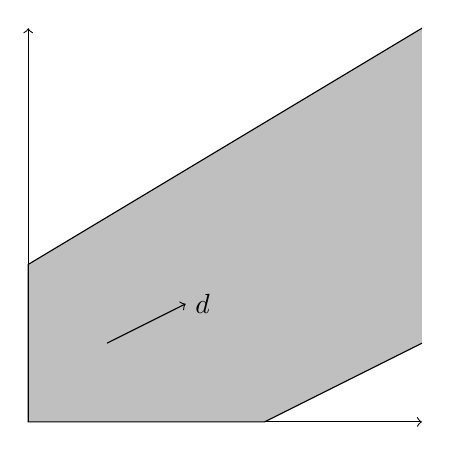
\begin{tikzpicture}

\draw[<->] (0,5) -- (0,0) -- (5,0);

\draw[fill=lightgray] (5,1) -- (3,0) -- (0,0) -- (0,2) -- (5,5);
\draw[->] (1,1) -- (2,1.5);
\node[right] at (2,1.5) {$d$};
\end{tikzpicture}
\caption{An unbounded polyhedron}
\end{figure}

\paragraph{}Observe that if $P$ is unbounded then the corresponding linear program may not have a finite optimal value. In particular this happens when translating along a direction $d$ can increase the objective value That is to say $P \neq \emptyset$, and there exists direction $d$ and objective function $c$ for which $c^Td >0$. By choosing successively larger $\alpha$ we may make the objective value of $x + \alpha d$ arbitrarily large. Linear programs whose feasible regions are polytopes always have finite optimal values. For the critical reader we refer you to Chvatal \cite{chvatal1983linear} for a proof.

\paragraph{}
Let $P$ denote the feasible region of a linear program of the form \ref{LP:standard} and let $x$ be a vector in $P$. Then $x$ is a {\it vertex} of $P$ if there exist $h$ and $\delta$ such that $h^Tx = \delta$ and for all $y \in P$
such that $y \neq x$ we have $h^Ty < \delta$. The hyperplane specified by $(h,\delta)$ is called a {\it supporting hyperplane} for $x$.

\paragraph{}In the same setting as the previous definition, we say $x$ is an {\it extreme point} if there do not exist distinct $y^1, y^2 \in P$ such that 
$$ x = \frac{1}{2} y^1 + \frac{1}{2}y^2.$$

\paragraph{}Again in the same setting, for ease of exposition let \begin{equation}A' = \begin{bmatrix} A \\ -I \end{bmatrix} \quad b' = \begin{bmatrix} b \\ 0 \end{bmatrix}\label{LP:augmented}\end{equation} and thus $P = \{x : A'x \leq b'\}$. The vector $x\in P$ is called a {\it basic feasible solution} if there exist $n$ linearly independent rows of $A'$, say $a_1, \dots, a_n$ (not necessarily the first $n$ rows of $A$), with corresponding entries of $b'$: $b_1, \dots, b_n$ satisfying $a_i x = b_i$ for all $i\in \{1,\dots, n\}$.

\paragraph{} It is not immediately obvious that the three concepts $x$ being a vertex, an extreme point, or a basic feasible solution are equivalent but in the next lemma we will show the surprising fact that they are indeed.

\begin{lemma} \label{lemma:bfs-equiv}Let $P$ be the polyhedron corresponding to the feasible region of $\ref{LP:standard}$, and let $x \in P$. Then the following are equivalent: 
\begin{enumerate}
\item $x$ is a vertex of $P$,
\item $x$ is an extreme point of $P$, 
\item and $x$ is a basic feasible solution of $P$.
\end{enumerate}
\end{lemma}
\begin{proof}
($(1) \implies (2)$) First suppose that $x$ is a vertex of $P$ with supporting hyperplane $h^T x = \delta$. Then $h^Ty < \delta$ for all $y \in P$ such that $y \neq x$. Suppose for a contradiction that $x$ is not an extreme point of $P$. Then there exist $y^1, y^2 \in P$ with $y_1 \neq y_2$, such that $$ x = \frac{1}{2}y^1 + \frac{1}{2}y^2.$$ So then $$\delta = h^T x = h^T(\frac{1}{2} y^1 + \frac{1}{2} y^2) = \frac{1}{2}h^Ty^1 + \frac{1}{2} h^Ty^2 < \frac{1}{2}\delta +\frac{1}{2}\delta = \delta,$$ yielding $\delta < \delta$, a contradiction. Thus $x$ is a vertex implies $x$ is an extreme point.
\paragraph{}
($(2) \implies (3)$) For ease of exposition let $A'$ and $b'$ be as in equations \ref{LP:augmented}. We proceed by contraposition. Suppose that $x$ is not a basic feasible solution. Then there are not $n$ linearly independent constraints tight at $x$. Let $k$ be the number of constraints satisfied by $x$ at equality. We may assume that the first $k$ rows of $A'$, $a_1, \dots, a_k$ along with the first $k$ entries of $b'$ describe the constraints $x$ satisfies at equality. Notice that either $k<n$, or $k\geq n$ and $a_1, \dots, a_k$ are not linearly independent. In either case the system (in variables $y$):
\begin{align*}
a_1^T y &= 0 \\
&\dots \\
a_k^T y &= 0
\end{align*}
has a non-trivial solution. Let $d \neq 0 \in \R^n$ be such a solution. Since adding or subtracting multiples of $d$ from $x$ does not affect satisfaction of tight constraints, and all other constraints satisfied by $x$ are not tight (that is, $a_i x < b_i$ for such constraints), there exists $\epsilon \neq 0$ such that $x+ \epsilon d, x-\epsilon d \in P$. Thus letting $y^1 = x+ \epsilon d$ and $y^2 = x-\epsilon d$ we have
$$\frac{1}{2}(y^1 + y^2) = \frac{1}{2}(2x) = x.$$
Since $y^1, y^2 \in P$ with $y_1 \neq y_2$, and $x = \frac{1}{2}y^1 + \frac{1}{2}y^2$, $x$ is not an extreme point. Thus we have shown that $x$ is extreme point implies that $x$ is a basic feasible solution.
\paragraph{}
($(3) \implies (1)$) Now suppose that $x$ is a basic feasible solution. Suppose that rows of $A'$, $a_1, \dots, a_n$, along with $b_1, \dots, b_n$ describe the linearly independent constraints satisfied by $x$ at equality. By linear independence, $x$ is the unique solution to 
$$\begin{bmatrix} a_1 \\ \vdots \\ a_n \end{bmatrix} x = \begin{bmatrix} b_1 \\ \vdots \\ b_n \end{bmatrix}.$$
Let $h^T = \sum_{i=1}^n a_i$ and let $\delta = \sum_{i=1}^n b_i$. We claim that $(h, \delta)$ describe a supporting hyperplane for $x$. Indeed let $y \in P$. Then 
$$ h^T y = \sum_{i=1}^n a_i y \leq \sum_{i=1}^n b_i$$
with the last inequality following since $y \in P$ implies $a_i y \leq b_i$ for all $i \in \{1, \dots, n\}$. Observe that equality holds above if and only if $a_i y = b_i$ for all $i\in\{1,\dots,n\}$. But since $x$ is the unique solution to the system of equations $a_i y = b_i$ for all $i\in\{1,\dots,n\}$ this implies that $y = x$ . Hence if $y \in P$ with $y \neq x$ then $h^T y < \delta$. Therefore $x$ is a basic feasible solution implies that $x$ is a vertex, and hence the lemma holds. 
\end{proof}

\begin{lemma}\label{lemma:rank}
(Rank Lemma \cite{lau2011iterative}) Let $x$ be an extreme point of $P$. If $x>0$ then there are $n$ linearly independent constraints tight at $x$ of the form $a_ix = b_i$, which is the maximum number possible. Here $a_i$ denotes a row of $A$ and $b_i$ is the entry of $b$ corresponding to $a_i$.  
\end{lemma}
\begin{proof}
By lemma \ref{lemma:bfs-equiv} we have that $x$ is a basic feasible solution. Hence there exist $n$ linearly independent constraints tight at $x$. Since $x>0$ each tight constraint is of the form $a_i x = b_i$ for some $i$, as no non-negativity constraints are tight. Therefore the row rank of $A$ is at least $n$. But $A$ is an $m \times n$ matrix, and thus the column rank of $A$ is at most $n$. Since it is a ubiquitous fact from linear algebra that column rank and row rank are equal for any matrix this implies that the row rank of $A$ is equal to $n$. Therefore $n$ is the maximal number of linearly independent constraints of the form, $a_i x = b_i$, tight at $x$.
\end{proof}

\begin{lemma} Let $x$ be an optimal solution to a linear program of the form \ref{LP:standard} with feasible region denoted by $P$. We claim there exists $x^* \in P$ such that $x^*$ is an extreme point and $c^Tx = c^Tx^*$.
\end{lemma}
\begin{proof}
Let $x$ be an optimal solution with the maximum number of constraints tight at $x$. Suppose for a contradiction that $x$ is not an extreme point. We will demonstrate that we can always find another optimal solution with more tight constraints than $x$ (possibly non-negativity constraints, which manifest as $0$-entries of $x$) contradicting our choice of $x$. Since $x$ is not an extreme point there exists $y^1, y^2 \in P$ with $y_1 \neq y_2$, such that  $$x = \frac{1}{2} y^1 + \frac{1}{2}y^2.$$
We define a direction $d\neq 0$ along which we will translate $x$ without ruining optimality. Let
$$ d = \frac{1}{2}y^2 - \frac{1}{2} y^1.$$
Then $x + d = y^2 \in P$ and $x - d = y^1 \in P$. We have the following inequalities
\begin{align*} A(x+d) &\leq b \\ x+d &\geq 0 \\
A(x-d) &\leq b \\ x-d &\geq 0 .\end{align*}
Let $A^=$ be the collection of rows of $A$ along with corresponding entries of $b$, $b^=$, that satisfy $A^= x = b^=$. So by the above inequalities $A^=(-d) \leq 0$ and $A^=d \leq 0$. Therefore $A^=d = 0$. Further, by the optimality of $x$,
\begin{align*}
c^Tx &\geq c^T(x+d) \\
\text{and } c^Tx &\geq c^T(x-d) \\
\text{which implies } c^Td = 0.
\end{align*}
Thus for any $\epsilon$, $x+\epsilon d$ satisfies $A^=(x+\epsilon d) = b^=$ and $c^T(x+\epsilon d) = c^Tx$. Since $d \neq 0$, we may assume that there exists $i$ such that $d_i < 0$ (otherwise we may use $-d$ instead of $d$). We define $\epsilon > 0$, which is finite as $d_i < 0$, as follows:
$$ \epsilon = \min\{ \min\{\frac{x_j}{-d_j}: d_j < 0\}, \min \{\frac{b_i - a_i x }{-a_id}: a_i x < b_i, a_i d < 0 \}\}.$$
where $a_i$ are the rows $A$ and $b_i$ is the corresponding entry of $b$. By our choice of $\epsilon$ either $x+\epsilon d$ has one more $0$ entry (in the $\frac{x_j}{-d_j}$ case) or one more tight constraint (in the $\frac{b_i-a_i x}{-a_id}$ case) than $x$. Further by the minimality of $\epsilon$ the non-tight constraints remain feasible, and as previously argued the tight constraints are not violated so $x + \epsilon d$ is feasible. Since $c^Td = 0$ we thus have $x + \epsilon d$ is an optimal solution with more tight constraints than $x$.
\end{proof}
\paragraph{Integrality}
The previous lemma tells us that an algorithm which solves linear programs need only concern itself with extreme point solutions. So extreme point solutions are of particular interest in applications. We call a polyhedron $P$ integral if every extreme point $x$ of $P$ is contained in $\Z^n$. We will call a linear program integral if its feasible region is integral. Integrality is important when using linear programs to model discrete optimization problems since fractional solutions rarely have an interpretation in this context. Later in this section we will demonstrate how iterative rounding can be used to prove that the feasible region of a linear program is integral.
\begin{figure}
\centering
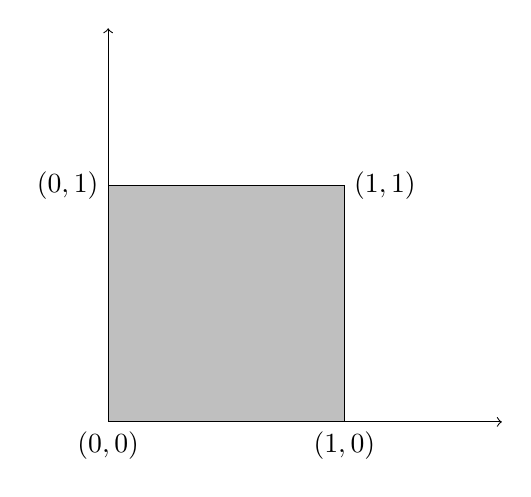
\begin{tikzpicture}
\draw[<->] (5,0) -- (0,0) -- (0,5);

\draw[fill=lightgray] (0,0) node[below]{$(0,0)$} -- (0,3) node[left]{$(0,1)$} -- (3,3) node[right]{$(1,1)$} -- (3,0) node[below]{$(1,0)$} -- (0,0);
\end{tikzpicture}
\caption{An integral polytope}
\small
\begin{flushleft}
This integral polytope has extreme points $(0,0)$, $(0,1)$, $(1,1)$, and $(1,0)$ which are all in $\{0,1\}^2\subseteq \Z^2$.
\end{flushleft}
\end{figure}
\paragraph{Algorithms for Linear Programming}
The most widely taught algorithm for solving linear programs is the simplex method\cite{dantzig1955generalized}. The algorithm works by starting at an extreme point and traveling along edges of the polyhedron given by the feasible region to adjacent extreme points which improve the objective value until the optimal solution is found. The order it chooses extreme points to visit is based on what is called a pivot rule. There is no known pivot rule which ensures that the simplex method examines a polynomial number of extreme points in the worst case. While this indicates a poor worst case performance for known implementations of the simplex method, it has been observed to work efficiently in practice possibly due to its average case polynomial time performance \cite{smale1983average}. The ellipsoid method came later, initially as an approximation algorithm for real convex minimization, and later shown to be able to solve linear programs in polynomial time \cite{grotschel1981ellipsoid}. While not thought to be faster than simplex in practice, the polynomial time worst case bound of the ellipsoid method is important for discrete optimization as it allows the use of linear programming for giving polynomial time algorithms for combinatorial problems,
\paragraph{Further Reading}
The theory of linear programming is rich and very well understood. One particularly important topic not mentioned here that one needs to know to truly understand linear programming is duality theory and complementary slackness. It studies the phenomenon that linear programs come in primal-dual pairs that are solved simultaneously, and the consequences surrounding this. Unfortunately this theory is outside the scope of this thesis, but we encourage the interested reader to see Chvatal \cite{chvatal1983linear} for a treatment of this topic. Its study is worthwhile for combinatorial optimizers as it has led to, among other ideas, the famous class of algorithms known as primal-dual methods.
\subsection{Strategy}
\paragraph{}
After our brief detour into the theory of linear programming, we are now ready to describe the method through which iterative rounding can be used to prove that a linear programming relaxation of a combinatorial optimization problem is integral. In this subsection we will describe the general approach at a high level, and in the following section we will apply this approach to bipartite matching to demonstrate the technical details. See the excellent monograph of Lau, Ravi, and Singh\cite{lau2011iterative} for other applications, and ways to extend this approach to giving approximation algorithms.
\paragraph{}
Since we wish to describe iterative rounding in general, we are going to need some terminology to formalize what we mean in general by a problem, a combinatorial optimization problem, residual problem instances, and linear programming relaxations. This may seem somewhat esoteric, but the goal is to capture the general principles common to iterative rounding approaches. For a more concrete treatment of iterative rounding as it pertains to maximum weight matching in bipartite graphs see the next subsection: \ref{subsec:irapp}

\paragraph{}We formalize the notion of a {\it problem} as a relation $R \subseteq \cI \times \cO$ where $\cI$ is some set of possible inputs, and $\cO$ is some set of possible outputs. The pair $(I,O) \in \cI \times \cO$ are related in $R$ if $O$ is a solution when given input instance $I$. We say that algorithm $\cA$ {\it solves} problem $R$ if $\cA$ takes inputs from $\cI$ and for every $I \in \cI$, running $\cA$ with input $I$ yields output $O$ such that $(I,O) \in R$. 

\paragraph{Example}
For example consider the maximum cardinality matching problem from subsection \ref{subsec:mcm}. In this problem we could say that $\cI$ is the set of all graphs, and $\cO$ is the set of all matchings of a graph. So if we let $R$ denote the maximum cardinality matching problem, $G$ denote a graph and $M$ denote a matching of $G$ then we can say $$(G,M) \in R \text{ if and only if for all matchings } M'\text{ of } G, \text{ we have } |M| \geq |M'|.$$
Moreover we have an algorithm, namely Edmonds Blossom algorithm \cite{edmonds1965paths}, which solves problem $R$.
\paragraph{Combinatorial Optimization Problems}
Generally speaking combinatorial optimization problems are problems wherein either implicitly or explicitly one is tasked with choosing an optimal subset $S \in \cS$ where $\cS$ is a family of feasible sets formed from elements of a discrete ground set $E$. In our previous example, the maximum cardinality matching problem satisfies this definitions of a combinatorial optimization problem. Namely given a graph $G$ as input then our ground set is $E(G)$, and our family of feasible subsets can be described implicitly as $\cS = \{M \subseteq E: |M \cap \delta(v)| \leq 1 \text{ for all } v\in V(G)\}$. Our optimal $M \in \cS$ is the matching which satisfies $|M| \geq |M'|$ for all $M' \in \cS$.
\paragraph{Step 1 - Linear Programming Formulation}
We are given some combinatorial optimization  problem $CP$ with ground set $E$ as an input instance to start. From this optimization problem instance we attempt to write a linear programming relaxation $LP(E)$. For $LP(E)$ to be a relaxation of this instance of $CP$, there must be a bijection between solutions of this instance of $CP$ and integral solutions of $LP(E)$. Classically this bijection is achieved via the mapping of subsets of $E$ to their corresponding incidence vectors (see $\chi$ in max weight matching section \ref{GT:MWM}). Such $LP(E)$ is called a relaxation because the optimal value of $CP(E)$ is bounded by the optimal value of $LP(E)$ and in the case that $LP(E)$ is integral the optimal values are equal.
\paragraph{}
In some applications the linear programming relaxation given in step $1$ will have an exponential number of constraints. In this situation it is not immediate that $LP(E)$ is solvable in polynomial time with respect to size of the input to $CP$. While this problem does not arise in the applications to matching we describe in this thesis, there are methods which may circumvent it. The ellipsoid method operates with a separation oracle \cite{grotschel1981ellipsoid}, which is a procedure that decides if a given point is feasible for the linear program, and in the case of infeasibility provides a hyperplane which separates the point from the feasible region. It is normal that the inequalities of $LP(E)$ have some implicit description in terms of the combinatorics of $CP$, and so it may be possible to give a polynomial time separation oracle despite having an exponential number of constraints needed to define $LP(E)$. If one can give such a separation oracle then $LP(E)$ is polynomial time solvable despite its exponential size.
\paragraph{}
In our upcoming description of a general iterative rounding procedure, we will refer to the concept of residual problem instances. What we are aiming to capture is the idea of being able to use solutions to smaller instances of a problem to solve a larger instance of a problem, for some appropriate notion of smaller and larger.

\paragraph{}Let $P \subseteq \cI \times \cO$ be a problem. Suppose that $\cI$ is equipped with some partial order $\leq$. Let $I, I' \in \cI$. If $I' \leq I$ then we say that $I'$ is a {\it residual problem instance} of problem instance $I$.

\paragraph{Example}
Consider once more the example of the maximum cardinality matching problem. Let $G, G'$ be graphs. We say $G'$ is a subgraph of graph $G$ if $V(G') \subseteq V(G)$ and $E(G') \subseteq E(G)$. The subgraph relation is a partial order on the space of all graphs. Hence we can say that $G'$ is a residual problem instance of $G$.
\paragraph{Step 2 - Iterative Algorithm}
Let $CP$ be a combinatorial optimization problem on ground set $E$. Let $LP(E)$ be a linear programming relaxation of $CP(E)$ for which the variables of our linear program are bounded between $0$ and $1$. The assumption that the feasible region of our linear programs is contained in $[0,1]^{|E|}$ is reasonable because such a case occurs naturally when using $\chi$ to map between solutions of $CP$ and integral solutions of $LP(E)$. 
\paragraph{}
In this step we describe an algorithm which constructs an integral optimal solution to $LP(E)$, which is equivalently a solution to $CP(E)$. The algorithm constructs integral optimal solution $x^*$ as follows:
\begin{enumerate}
\item Let $x$ be an optimal extreme point solution of $LP(E)$.
\item For each $e \in E$ for which $x_e  \in \{0,1\}$ set $x^*_e = x_e$ and remove $e$ from $E$.
\item If $E$ is now empty return $x^*$ and terminate.
\item Otherwise repeat from step 1.
\end{enumerate}
Observe that if the algorithm always finds $x_e \in \{0,1\}$ then $|E|$ decreases at every iteration and thus the algorithm terminates. What the algorithm is doing intuitively is finding variables which are integral in an extreme point solution, fixing them to their corresponding values in the solution it will return, then removing those variables from the ground set resulting in a residual problem. The algorithm then iterates, considering an optimal solution for the residual problem. 
\paragraph{}
The following lemma explains how an algorithm can be used to prove the integrality of a polytope. This lemma indicates the properties we will need to prove our algorithm satisfies in order for its existence to imply that $LP(E)$ is integral.
\begin{lemma} If there exists an algorithm $\cA$ that always returns an integral optimal solution to $LP(E)$ for any objective function $c$, and terminates then the feasible region of $LP(E)$ is integral.
\end{lemma}
\begin{proof}
We may assume without loss of generality that $LP(E)$ is a maximization problem. Let $x$ be an extreme point of $P$, the feasible region of $LP(E)$. Then $x$ is equivalently a vertex of $P$ by lemma \ref{lemma:bfs-equiv}. So there exists a supporting hyperplane described by $(h,\delta)$ for which $h^Tx = \delta$ and for all $x' \in P$ with $x' \neq x$, we have $h^Tx' < \delta$. If we consider the linear program $LP(E)$ with objective function $h$ then $x$ is the unique optimal solution of this linear program. Therefore if we run algorithm $\cA$  with objective function $h$ as input then the integral solution returned is equal to $x$ by uniqueness. Thus $x$ is integral, and so any extreme of $P$ is integral. 
\end{proof}
\paragraph{Step 3 - Algorithm Analysis}
We need to establish two things in this phase: that the algorithm terminates in finite time giving an integral vector and that it indeed returns an optimal solution.
\subparagraph{Termination} Recall that we are assuming that the feasible region of $LP(E)$ is contained in $[0,1]^{|E|}$. To show that the algorithm terminates we demonstrate that there always exists an $e$ for which $x_e \in \{0,1\}$ for every iteration. Doing so proves inductively that the algorithm terminates with a $\{0,1\}$ valued vector. There is a standard approach to showing the existence of $x_e \in \{0,1\}$ which proceeds by contradiction. If we suppose that every $x_e$ lies in the interval $(0,1)$ then we may obtain a contradiction as follows. Since $x>0$ we may invoke lemma \ref{lemma:rank} saying there exists a maximal set of $|E|$ linearly independent constraints not drawn from non-negativity constraints which are tight at $x$. If we can then show an upper bound on the number of linearly independent constraints tight at $x$ that is smaller than $|E|$, then we have obtained a contradiction as desired. This will become more concrete in the next section when we demonstrate an example.
\subparagraph{Correctness} It remains to show that the algorithm returns an optimal solution. For iterative algorithms this typically takes the form of an inductive argument on $|E|$. We show two things:
\begin{enumerate}
\item the vector $x$ restricted to the variables in the residual problem instance is feasible for the linear programming relaxation of the residual problem instance,
\item and the integral optimal solution to the linear programming relaxation of the residual problem instance, along with the variables which were previously fixed to $0$ or $1$ in step $2$ of the current iteration is a feasible solution to $LP(E)$.
\end{enumerate}
Together this allows one to conclude that the objective value at $x$ is at most that of the integral solution returned by the algorithm. Since $x$ is optimal this implies that the integral solution returned has the same objective value as $x$ and is thus optimal.
\subsection{Application to Matching}\label{subsec:irapp}
\paragraph{}
Recall the linear programming relaxation of maximum weight matching in bipartite graphs which we will denote $LP(G)$ for a given bipartite graph $G$:
\begin{align*}
	&\text{max} \sum_{e \in E(G)} w(e) x_e \\
	&\text{s.t.} \sum_{e \in \delta(v)} x_e \leq 1 &\text{for all $v \in V(G)$} \\
	&\quad\quad\quad\ \ x_e \geq 0 &\text{for all $e \in E(G)$.}
\end{align*}
\paragraph{}
We will use iterative rounding to prove that this linear program is integral. Consider an iterative rounding algorithm for bipartite matching with weighted input graph $G$.
\begin{enumerate}
\item Set $M \leftarrow \emptyset$
\item While $|E(G)| > 0$\begin{enumerate}
\item Let $x$ be an extreme point optimal solution to $LP(G)$.
\item For each edge $e$ with $x_e = 1$: $M \leftarrow M \cup \{e\}$.
\item For each edge $e$ with $x_e \in \{0,1\}$ : $G \leftarrow G - e$.
\end{enumerate}
\item return $M$
\end{enumerate}
It is important to note that the linear program in step $2(a)$ needs only be solved once, during the first iteration, to obtain $x$. This is because the original extreme point $x$ remains an extreme point for each subsequent iteration's linear programming relaxation when restricted to the appropriate variables.
\paragraph{}
To prove that $LP(G)$ is integral for any weighted bipartite graph $G$ we need to show that our iterative algorithm always terminates in finite time and returns an integral solution of optimal value.
\paragraph{} Since our graph $G$ is finite, demonstrating termination is simply a matter of verifying that for any extreme point solution $x$ of $LP(G)$ there exists an edge $e$ with $x_e \in \{0,1\}$. In doing so we will need the following lemma about extreme points of $LP(G)$.
\begin{lemma}\label{lemma:extreme-point-characterization} Let $x$ be an extreme point optimal solution to $LP(G)$. Suppose that for all $e \in E(G)$, $x_e > 0$. Then there exists $W \subseteq V(G)$ satisfying
\begin{itemize}
\item $\sum_{e\in\delta(v)} x_e = 1$ for all $v \in W$ \\
\item $\{\chi(\delta(v)) : v \in W\}$ is linearly independent (recall that $\chi : E(G)\rightarrow \{0,1\}^{|E(G)|}$ maps edge sets to incidence vectors)
\item $|W| = |E(G)|$.
\end{itemize} 
\end{lemma}
\begin{proof}
The proof is immediate from lemma \ref{lemma:rank}.
\end{proof}
\paragraph{} We will now prove that our iterative rounding algorithm always terminates returning a matching (equivalently an integral solution). We will do this via a contradiction argument proving that a $0,1$ variable can always be found.
\begin{lemma} Let $x$ be an optimal extreme point solution to $LP(G)$. Then there exists $e \in E(G)$ such that $x_e \in \{0,1\}$.
\end{lemma}
\begin{proof}
Suppose for a contradiction that for all $e\in E(G)$, $0 < x_e < 1$. By lemma \ref{lemma:extreme-point-characterization} there exists $W \subseteq V(G)$ containing vertices corresponding to $|E(G)|$ linearly independent tight vertex constraints. Let $v \in W$. Since $\sum_{e\in \delta(v)} x_e = 1$ and $x_e < 1$ for all $e$, we have $d(v) \geq 2$. So then
$$2|W| = 2|E(G)| = \sum_{v \in V(G)} d(v) \geq \sum_{v\in W} d(v) \geq 2|W|.$$
The inequalities above thus hold as equalities. Since $\sum_{v\in V(G)} d(v) = \sum_{v \in W} d(v)$, $d(v) = 0$ for all $v \not\in W$. Since $\sum_{v \in W} d(v) = 2|W|$ we have $d(v) = 2$ for all $v \in W$. Therefore $E(G)$ is a set of cycles covering the vertices of $W$, which is to say each vertex is contained in an edge of $E(G)$ and the edges of $E(G)$ form cycles. Let $C \subseteq E(G)$ be a cycle with $V(C) \subseteq W$. Let $V_1, V_2$ be a bipartition of the vertex set of $G$ (which exists since $G$ is bipartite). Further since $G$ is bipartite for each edge $vw \in E(C)$ one of $v,w $ is in $V_1$ and the other is in $V_2$. Hence we have
$$\sum_{v \in V(C) \cap V_1} \chi(\delta(v)) = \sum_{v\in V(C) \cap V_2} \chi(\delta(v))$$
which contradicts the linear independence of $\{\chi(\delta(v)) : v \in W\}$.
\end{proof}
\paragraph{}
It remains to verify that our algorithm returns an optimal solution. We show that via an inductive argument in the following lemma.
\begin{lemma}
The iterative rounding algorithm returns a matching of weight at least that of an optimal solution $LP(G)$.
\end{lemma}
\begin{proof}
We proceed by induction on the number of iterations the algorithm runs to solve the problem. In the base case if the algorithm runs for a single iteration then the returned solution is exactly the incidence vector of an extreme point optimal solution to $LP(G)$. That is, the lemma holds trivially. So for induction suppose the algorithm needs $k$ iterations to return an answer for input graph $G$ and for any graph $G'$ such that the algorithm needs less than $k$ iterations to solve the problem, the algorithm returns an optimal matching. Let $x$ be the extreme point of $LP(G)$ found in step $2(a)$. Let $R$ be the set of edges removed in step $2(c)$ of the algorithm when run on $G$. Let $G'$ be the residual graph ($G$ restricted to edges $E(G) \backslash R$). The next iterations of the algorithm are equivalent to simply running the algorithm on $G'$. Let $M'$ be the matching returned. By the inductive hypothesis $w(\chi(M')) \geq w(x')$ for any $x'$ feasible for $LP(G')$. Let $x'$ be the point $x$ restricted variables corresponding to edges in $E(G')$. Then $w(x) = w(x') + w(\chi(R))$. Further, as $x'$ is feasible for $LP(G')$, we have
$w(\chi(M')) \geq w(x')$. Let $M$ be the matching returned. Then $M = M' \cup R$ and thus
$$w(\chi(M)) = w(\chi(M')) + w(\chi(R)) \geq w(x') + w(\chi(R)) = w(x).$$
Therefore by induction the algorithm always returns a matching with weight at least that of an optimal solution to $LP(G)$. 
\end{proof}
\paragraph{}
As discussed in the previous section, the above lemmas imply that that $LP(G)$ is integral.
\section{Stable Matching}\label{sec:SM}
\subsection{Problem}
\paragraph{Input}The stable matching problem gives as input a bipartite graph $G=(V, E)$ with bipartition $V = A\cup B$, where each $v \in V$ has a strict order over $\delta(v)$ referred to as $v$'s preferences. We will use $u <_v w$ to denote that edge $vw$ is preferred by $v$ to edge $vu$, and we will use $>_v$, $\leq_v$, $\geq_v$, and $=_v$ analogously. We say equivalently that $v$ prefers $w$ to $u$ and can treat $<_v$ as an order on the vertices adjacent to $v$. It will usually be clear from context how we are viewing $<_v$.
\paragraph{Output} Given a stable matching instance as input with underlying graph $G$ one is to find a matching $M$ in $G$ that is stable. A matching is called stable if there is no blocking pair $(a,b)$. A pair $(a,b)$ is said to block $M$ if $ab \not\in M$ and $b >_a M(a)$ and $a >_b M(b)$.
\paragraph{Application} The sets $A,B$ are colloqially referred to as men and women respectively. This alludes to the toy application of stable matching in forming couples from single people together who have preferences over the opposite gender. In this context a blocking pair references to a pair who mutually prefer each other to their partner. One of the original applications of stable matching \cite{roth1984evolution} was to pair medical students with hospitals at which they were to do their residency, and another was college admissions.
\subsection{Gale Shapley Algorithm}\label{SM:ALG}
\paragraph{}
In their original work, Gale and Shapley gave an algorithm, called deferred acceptance \cite{gale1962college}, for solving the stable matching problem and in doing so proved that every bipartite graph with strict preference orders has a stable matching.
\paragraph{Deferred Acceptance Algorithm}
In the following description of the algorithm we adopt the convention that vertices prefer to be matched than to be unmatched. For each vertex in $a\in A$ we maintain a set $P(a)$ of vertices in $B$ that $a$ has previously ``proposed" to. Given an input graph $G=(A \cup B, E)$ with preferences do:
\begin{enumerate}
\item Assign $M \leftarrow \emptyset$
\item Assign $P(a) \leftarrow \emptyset$ for all $a \in A$
\item While there exists $a \in A$ such that $a \not\in V(M)$ and $P(a) \neq \{b \in B : a\sim b\}$:
	\begin{enumerate}
	\item Let $b$ be such that $b \geq_a b'$ for all $b' \in \delta(v) \backslash P(a)$
	\item Assign $P(a) \leftarrow P(a) \cup \{b\}$
	\item If $a >_b M(b)$ then assign $M \leftarrow M \cup \{ab\} \backslash \{M(b)b\}$
	\end{enumerate}
\item Return $M$.
\end{enumerate}
\begin{lemma} Deferred Acceptance returns a matching.
\end{lemma}
\begin{proof}
From step $3(c)$ it is clear that each $b \in B$ is matched to at most one $a \in A$. Further any $a \in A$ matched in step $3(c)$ is unmatched by the While condition of step $3$, and hence each $a \in A$ is matched to at most one $b \in B$. Therefore $M$ returned is a matching. \end{proof}
\begin{theorem}(Gale-Shapley): The matching returned by Deferred Acceptance is stable.
\end{theorem}
\begin{proof}
We claim that Deferred Acceptance maintains the following invariant: at any iteration for any $a \in A$ for all $b \in P(a)$, $M(b) \geq_b a$. We prove this claim by induction. In the base case, at the start of the algorithm $P(a) = \emptyset$ for all $a \in A$ and hence the claim is vacuously true. In the inductive case consider some iteration of the algorithm. Let $a\in A$ be the vertex chosen in step $3$. Let $b \in B$ be as chosen in step $3(a)$. In step $3(b)$, $b$ is added to $P(a)$. By induction the invariant holds for all $b' \in P(a)$ except $b$. In step $3(c)$ if $a \leq_b M(b)$ then the invariant holds for $b \in P(a)$ and no changes are made. If $a >_b M(b)$ then $b$ is matched to $a$ and hence after step $3(c)$ the invariant holds for $b$ and thus the entirety of $P(a)$. For all other $a' \neq a$, $P(a')$ is unchanged and hence by induction the invariant holds for all $b' \in P(a')$ except $b$. So consider if $b \in P(a')$. Observe that $a$ is preferred by $b$ to her match prior to this iteration and hence by transitivity the invariant also holds for $b \in P(a')$. Therefore by induction the invariant holds. It is easy to see from step $3$ that the algorithm also maintains the invariant that for all $b \in \delta(a)\backslash P(a)$, $M(a) \geq_a b$. Hence if $ab \in E$ with $ab \not\in M$ at termination of the algorithm then either $b \in P(a)$ or $b \not\in P(a)$. If $b \in P(a)$ then $M(b) >_b a$ (as $a \neq M(b)$) and so $ab$ is not a blocking pair. If $b \not\in P(a)$ then as $ab \in E$, $b \in \delta(a) \backslash P(a)$ and so $M(a) >_a b$ (as $b \neq M(a)$). Therefore in either case $ab$ does not block $M$. Therefore $M$ is stable.
\end{proof}
\subsection{Structure}\label{SM:STRUCTURE}
\paragraph{}
Over time a rich body of literature around the structure of the set of stable matchings for certain families of bipartite graphs with preferences has been developed \cite{roth1992two}. In this subsection we will explore some of these results that will come up in our chapter on stable matching polytopes.

\paragraph{}
We say a stable matching $M$ is $A$-{\it optimal} with respect to our problem instance if for every stable matching $M'$ in this problem instance and for every $a \in A$, $M(a) \geq_a M'(a)$. That is, every man in $A$ likes $M$ at least as well as they like any other stable matching. We can define $B$-optimal analogously. Gale and Shapley showed that not only do $A$-optimal and $B$-optimal stable matchings exist in any problem instance, but also that their Deferred Acceptance algorithm computes an $A$-optimal stable matching \cite{gale1962college} (and could compute $B$-optimal matching by switching roles of $A$ and $B$).

\begin{theorem} (Gale and Shapley): For any bipartite graph $G = (A\cup B, E)$ with strict preferences there always exists a unique $A$-optimal ($B$-optimal analogously) stable matching and it can be computed via the Deferred Acceptance algorithm.
\end{theorem}
\begin{proof}
For any $v \in A\cup B$ let $$C(v) = \{w \in V(G) : w \sim v \text{ and there exists stable matching } M, w = M(v) \}$$ be the set of partners $v$ has a chance of being matched to in a stable matching. We will show that no $a \in A$ is ever rejected by any $b \in C(a)$ during the operation of Deferred Acceptance and hence since each $a \in A$ proposes to their most preferred choice in $C(a)$ before any other vertex in $C(a)$ the resulting matching is $A$-optimal. The uniqueness is achieved since the preferences are strict. We proceed by induction on the number of iterations Deferred Acceptance has run. In the base case no proposals and hence no rejections have yet happened. So consider the inductive case. Suppose that at the given iteration $b$ rejects $a$ (that is, either $a$ is unsuccessful in proposing to $b$ or $b$ leaves $a$ for a better proposer at this step). Let $a' \neq a$ be the vertex $b$ is matched to at the end of step $3(c)$ of the iteration under consideration. Then $a' >_b a$. By our induction hypothesis $P(a') \cap C(a') = \{b\}$ as $a'$ has not been rejected by any $b' \in C(a')$. Let $M$ be a matching formed by matching $a$ to $b$ and matching every other $v$ to a vertex in $C(v)$. Then $b >_{a'} M(a')$ as $b$ is the most preferred vertex of $a'$ in $C(a')$. Further $a' >_b a=M(b)$, and thus the pair $(a',b)$ blocks $M$. Since $(a',b)$ blocks any such matching $M$, $b \not\in C(a)$ (as otherwise we could form a stable matching $M$ matching $a$ to $b$). Hence the claim holds by induction, and we have proven the theorem. \end{proof}

\paragraph{} Knuth took the above idea a step further to show that the interests of $A$ and $B$ are opposed to each other. 

\begin{theorem} (Knuth) \cite{knuthmariages}:Let $M$ and $M'$ be two stable matchings for some problem instance. Let $M \geq_A M'$ denote that for all $a \in A$, $M(a) \geq_a M'(a)$. Define $M \geq_B M'$ analogously. We have that $M \geq_A M'$ if and only if $M' \geq_B M$.
\end{theorem}
\begin{proof}
Suppose $M \geq_A M'$. We will show that $M' \geq_B M$ since the other direction is symmetric about the roles of $A$ and $B$. Suppose for a contradiction that there exists $b \in B$ for which $M(b) >_b M'(b)$. Let $a = M(b)$. Then $M'(b) \neq M(b)$ and thus $M'(a) \neq M(a)$ as otherwise $b$ has two matches in $M'$. Since $M \geq_A M'$ and $M(a) \neq M'(a)$, $b=M(a) >_a M'(a)$. That is we have $a >_b M'(b)$ and $b >_a M'(a)$ and thus $(a,b)$ blocks $M'$. So $M'$ is not a stable matching, a contradiction. \end{proof}

\begin{corollary}For each $b \in B$, let $$C(b) = \{a \in A: \text{there exists stable matching }M, a = M(b)\}.$$ Let $\ell(b) \in C(b)$  be the vertex satisfying that for all $a \in C(b)$, $a \geq_b \ell(b)$. Then the $A$-optimal stable matching matches each $b \in B$ to $\ell(b)$. Note that this also holds by symmetry by exchanging the roles of $A$ and $B$.
\end{corollary}

\paragraph{}
These theorems begin to point towards an interesting structure for the set of stable matchings of a given problem instance. It was first observed by Conway \cite{knuthmariages} that this set forms an algebraic structure called a lattice. For those unfamiliar with lattices in this context we will proceed by explaining all the terms necessary to continue.

\paragraph{}Let $L$ be a set endowed with a partial order $\geq$. The set $L$ is said to be a {\it lattice} if for any $x, y \in L$ there exists a unique $sup(x,y) \in L$ such that $sup(x,y) \geq x,y$ and for every $z$ with $z \geq x,y$ we have $z \geq sup(x,y)$. Similarly there exists a unique $inf(x,y) \in L$ such that $x,y \geq inf(x,y)$ and for every $z$ with $x,y \geq z$ we have $inf(x,y) \geq z$. A lattice is said to be {\it complete} if each $X \subseteq L$ also has functions $sup$ and $inf$. 

\paragraph{Lattice functions for stable matchings} We now describe functions that will behave as $sup$ and $inf$ for stable matchings. Let $M, M'$ be any two stable matchings for a given problem instance. Let $M^* = sup(M,M')$ be given as follows. For all $a \in A$, $M^*(a) = M(a)$ if $M(a) >_a M'(a)$ and $M^*(a) = M'(a)$ otherwise. For all $b \in B$, $M^*(b) = M(b)$ if $M(b) <_b M'(b)$ and $M^*(b) = M'(b)$ otherwise. We can define $inf(M,M')$ analogously by interchanging the roles of $A$ and $B$. Intuitively $sup$  presents each $a \in A$ with a choice between their partner in $M$ and partner in $M'$ and pairs them with their preferred choice. In the next theorem we need to show $sup$ and $inf$ map to stable matchings and respect the partial order $\geq_A$.
\begin{theorem}(Conway)\label{theorem:lattice} \cite{knuthmariages}: The set of stable matchings for a given problem instance endowed with the partial order $\geq_A$ is a lattice via the functions $sup$ and $inf$ defined above.
\end{theorem}
\begin{proof}
We will demonstrate that $sup$ behaves as desired and note that the argument is symmetric about the roles of $A$ and $B$ for $inf$. Let $M, M'$ be stable matchings. It is clear from the construction of $sup(M,M')$ that  $sup(M,M')$ is unique and $sup(M,M') \geq_A M$ and $sup(M,M') \geq_A M'$ provided that $sup(M,M')$ is a stable matching. Further if $Z$ is a stable matching such that $Z \geq_A M, M'$ then for any $a \in A$, $Z(a) \geq_a M(a),M'(a)$. So $Z(a) \geq_a sup(M,M')(a)$ (since $Z(a) \in \{M(a), M'(a) \}$) and thus $Z \geq_A sup(M,M')$. Therefore it remains to show that $sup(M,M')$ is a stable matching.
\paragraph{}
Let $M^* = sup(M,M')$. We first show that $M^*$ is a matching and then verify stability. To show that $M^*$ is a matching we will prove that $M^*(a) = b$ if and only if $M^*(b) = a$. First, for sufficiency, suppose that $M^*(a) = b$.  We may assume without loss of generality that $b = M(a)$. Then $b \geq_a M'(a)$. Since $M'$ is stable, $a \leq_b M'(b)$ and hence $M^*(b) = a$ as desired. Now to show necessity suppose that $M^*(b) = a$. We may assume that $a = M(b)$. So $a \leq_b M'(b)$. Again by the stability of $M'$, $b \geq_a M'(a)$. So $M^*(a) = b$ as desired. Therefore $M^*$ is a matching. 
\paragraph{}
Now to see stability. Suppose for a contradiction that $ab$ blocks $M^*$. Then $b >_a M^*(a)$ and thus $b>_a M(a)$ and $b >_a M'(a)$. Also $a >_b M^*(b)$. So if $M^*(b) = M(b)$ then $ab$ blocks $M$ and if $M^*(b) = M'(b)$ then $ab$ blocks $M'$. Therefore in either case we have  a contradiction. \end{proof}
\paragraph{Further Reading}
The set of stable matchings of a given graph with preferences has been widely studied in academic literature. We have covered here the results key to our work in the following chapter, but many more interesting results are known. For instance, another interesting result to study is the surprising equivalence between distributive lattices and sets of stable matchings that we only began to set the stage for here. To read more on these things we recommend the survey text of Roth and Sotomayor\cite{roth1992two}.